\documentclass[12pt,a4paper]{article}
\usepackage{graphicx}
\usepackage[german]{babel}
\usepackage{float}





%\usepackage{geometry}
%\geometry{a4paper, margin=2cm}

\title{Dokumentation: Kollisionsdetektion, WPF-Projekt in SSDS}
\author{Ivan Kurilin \and Dimitrij Pivovar}
\date{\today}

\begin{document}
	\maketitle
	\begin{center}
		\textit{Technische Hochschule Köln }\\		
		\textit{Prof. Herr Dr. Konen}
	\end{center}
	\section{Einführung}	
	\subsection{Projektziel}
	
Das Ziel dieses WPF-Projekts war es, eine Kollisionsdetektion in einer 3D-Umgebung zu implementieren. Die Objekte sollten eine realistische Reaktion auf Kollisionen mit den Bällen zeigen und dem Benutzer verschiedene Methoden zur Veranschaulichung bieten, um die Kollisionen näher zu betrachten und besser zu verstehen.
	
	\subsection{Überblick}
	
Für die Entwicklung des Projekts stand uns eine einfachere Version in Processing zur Verfügung. In dieser wurden gleichmäßig bewegte Bälle im Raum simuliert, die nur mit den Wänden kollidieren konnten. Auf dieser Grundlage haben wir ein Projekt entwickelt, bei dem nicht nur die Kollisionen sichtbar sind, sondern dem Benutzer auch eine benutzerfreundliche Oberfläche, Funktionen zur Visualisierung und Optimierungsalgorithmen bereitgestellt werden.
	
	\section{Benutzeroberfläche}
	\subsection{Design}
	Dem User wird eine benutzerfreundliche Oberfläche angeboten, die man ganz einfach durch die Menüpunkte navigieren kann. 
	
	\subsection{Funktionen}
	\begin{itemize}
		\item \textbf{Normalmodus}:\\
		Dies ist die Grundlage des Projekts. Hier kann der Benutzer sehen, wie das Programm zu Beginn war.
		
		\item \textbf{Kollisionsdetektion (Bruteforce)}:\\
		Eine einfache Überprüfung auf Kollisionen mittels Bruteforce mit einer Laufzeit von O(n²).
		
		\item \textbf{Impuls Demonstration}:\\
		In diesem Modus hat der Benutzer die Möglichkeit, per Mausklick auf die Bälle zu klicken. Das Ziel dieses Modus ist es, zu verdeutlichen, welchen Einfluss die Masse auf die Kollision mit anderen Bällen hat, die weniger Masse besitzen.
		
		\item \textbf{Tunneling Demonstration}:\\
		In diesem Modus wird der quantenmechanische Tunneleffekt simuliert. Dies veranschaulicht das Phänomen, bei dem Teilchen eine Barriere durchqueren können, die sie gemäß klassischer Physik nicht passieren könnten.
		
		\item \textbf{Vektorenrichtung Drawer}:\\
		Dieser Effekt zeichnet Pfeile, die in die Bewegungsrichtung der Bälle zeigen.
		
		\item \textbf{Effet}:\\
		Dieser Modus ermöglicht es, die Rotation des Balls zu betrachten.
		
		\item \textbf{Quadtree Algorithmus}:\\
		Der Quadtree Algorithmus verbessert die Performance der Kollisionsdetektion. Durch die hierarchische Unterteilung des Raumes in vier Teilbereiche pro Knoten können Kollisionen effizienter erkannt werden. Die Laufzeit für das Einfügen eines Elements in einen Quadtree beträgt O(log(n)).
	\end{itemize}
	
	\section{Physikalische Grundlagen}
	\subsection{Elastische Kollision}	
	Wir bezeichnen einen Stoß dabei als elastisch, wenn die Summe der kinetischen Energien der Stoßpartner nach dem Stoß genau so groß ist wie vor dem Stoß. [1] \\
	Das bedeutet für uns, dass keine kinetische Energie in andere Energieformen wie Wärme oder Verformungsenergie umgewandelt wird. Ein klassisches Beispiel für eine nahezu elastische Kollision ist der Zusammenstoß von Billardkugeln: Nach dem Stoß bewegen sich die Kugeln mit nahezu unveränderter kinetischer Energie weiter.\\ Im Gegensatz dazu steht die unelastische Kollision, bei der ein Teil der kinetischen Energie in andere Energieformen umgewandelt wird, was oft zu einer dauerhaften Verformung der Objekte führt. Ein typisches Beispiel hierfür ist ein Autounfall, bei dem die kinetische Energie in Verformungsenergie umgewandelt wird, was zu Schäden am Fahrzeug führt.
	
	\vspace{0.5cm}
	
Um eine Kollision festzustellen, ist dies bei einer Ballkollision relativ einfach. Dafür benötigen wir die Distanz zwischen den beiden Bällen. Wenn diese Distanz kleiner ist als die Summe der Radien der Bälle, findet eine Kollision statt.

\begin{figure}[H]
	\centering 
	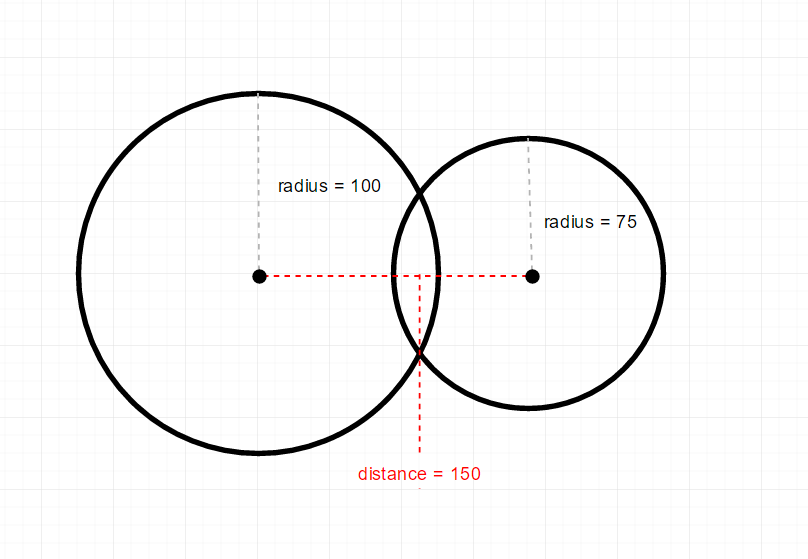
\includegraphics[width=0.8\textwidth]{collision-detection-6.png}  % Adjust the width as needed
	\caption{Kollision} 
	\label{Bild: Kollision}  
\end{figure}



	
	
		\subsection{Impuls und Impulserhaltungssatz}
		Die folgende Gleichung, bekannt als Impulserhaltungsgesetz stellt die Erhaltung der kinetischen Energie bei einem elastischen Stoß zwischen zwei Körpern dar.
		
		\[
		m_1 v_1^2 +  m_2 v_2^2 =  m_1 v_1'^2 +  m_2 v_2'^2
		\]
		
		\begin{itemize}
			\item \( m_1 \) und \( m_2 \) sind die Massen der Körper.
			\item \( v_1 \) und \( v_2 \) sind die Geschwindigkeiten der Körper vor dem Stoß.
			\item \( v_1' \) und \( v_2' \) sind die Geschwindigkeiten der Körper nach dem Stoß.
		\end{itemize}
		\subsection{Effet}
	
	\section{Algorithmen zur Kollisionsdetektion}
	
	\subsection{Bruteforce}
	Vor- und Nachteile
	\subsection{Quad-Tree}
	Vorteile gegenüber Bruteforce
	
	\section{Visualisierungen und Demonstrationen}
	
	\subsection{Vektorenrichtung Drawer}
	
	\subsection{Tunneling-Demonstration}
	
	
	\subsection{Impuls-Demonstration}
	
	\subsection{Effet}
	
	\section{Fazit }
	\section{Quellen}
	[1]: https://www.leifiphysik.de/mechanik/impulserhaltung-und-stoesse/grundwissen/zentraler-elastischer-stoss
	[2]: https://happycoding.io/tutorials/processing/collision-detection

	
	
	
	
	
\end{document}










\end{document}
